%tag:000X
%label:"fig:quadraticHamiltonian"
%author:JeffHicks
%name:"quadratic Hamiltonian"
%type:"figure"
%parent:con:symplecticCohomologyQuadratic
%caption:"An increasing Hamiltonian over the symplectization witnesses all Reeb orbits"


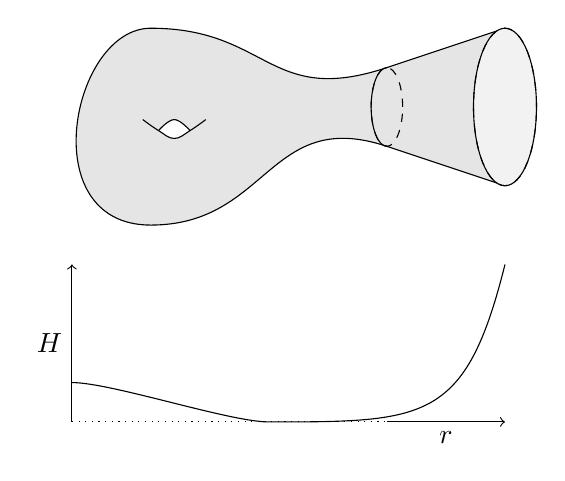
\begin{tikzpicture}
    \draw[fill=gray!20] (4,-0.5) .. controls (2.5,-1) and (4,-0.5) .. (2.5,-1) .. controls (1,-1.5) and (1,-0.5) .. (-0.5,-0.5) .. controls (-1.5,-0.5) and (-2,-3) .. (-0.5,-3) .. controls (1,-3) and (1,-1.5) .. (2.5,-2) .. controls (4,-2.5) and (2.5,-2) .. (4,-2.5);
    \begin{scope}[shift={(3.2,-2)}]
    
    \fill[white]  plot[smooth, tension=0.7] coordinates { (-3.6,0.2) (-3.4,0.1) (-3.2,0.2) }  plot[smooth, tension=0.7] coordinates {(-3.6,0.2) (-3.4,0.34) (-3.2,0.2)};
    
    \draw  plot[smooth, tension=0.7] coordinates {(-3.8,0.34) (-3.6,0.2) (-3.4,0.1) (-3.2,0.2) (-3,0.34)};
    \draw  plot[smooth, tension=0.7] coordinates {(-3.6,0.2) (-3.4,0.34) (-3.2,0.2)};
    
    
    
    \end{scope}
    
    \begin{scope}[]
    
    \draw[dashed]  (2.5,-1.5) ellipse (0.2 and 0.5);
    \clip  (2,-1) rectangle (2.5,-2);
    
    \draw  (2.5,-1.5) ellipse (0.2 and 0.5);
    \end{scope}
    
    \begin{scope}[scale=2, shift={(-0.5,0.75)}]
    
    \draw[dashed, fill=gray!10]  (2.5,-1.5) ellipse (0.2 and 0.5);
    
    
    \draw  (2.5,-1.5) ellipse (0.2 and 0.5);
    \end{scope}
    
    \draw[dotted] (-1.5,-5.5) -- (2.5,-5.5);
    \draw[->] (2.5,-5.5) --node[below]{$r$} (4,-5.5);
    \draw (-1.5,-5) .. controls (-1,-5) and (0.5,-5.5) .. (1,-5.5) .. controls (3,-5.5) and (3.5,-5.5) .. (4,-3.5);
    
    \draw[->] (-1.5,-5.5) -- node[left]{$H$} (-1.5,-3.5);
    \end{tikzpicture}